\section{Projektverlauf}
\label{sec:einleitung.Projektverlauf}

Die Projektarbeit richtete sich nach folgendem Zeitplan:

\begin{figure}[H]
\centering
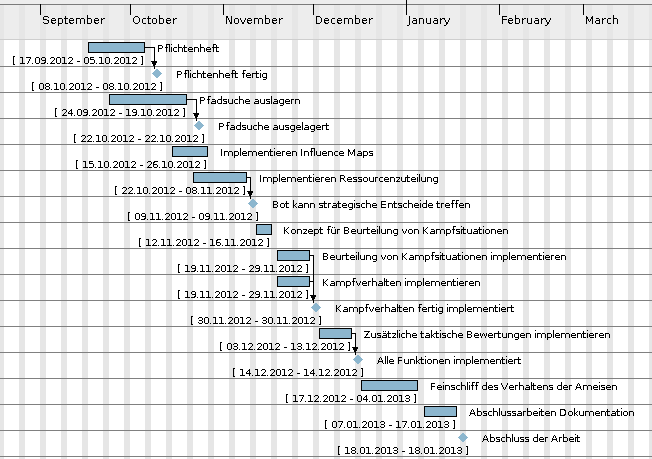
\includegraphics[width=0.9\textwidth]{91_bilder/gantt.png}
\caption{Projektablauf}
\label{fig:gantt}
\end{figure}

Dieser Zeitplan konnte mit lediglich geringen Abweichungen eingehalten werden, weshalb ein detaillierter Soll/Ist Vergleich hier wenig Sinn macht. Folgende Punkte sollen der Vollst�ndigkeit halber dennoch festgehalten werden:

\begin{itemize}
\item Obwohl die meiste Arbeit f�r bestimmte Aufgaben (z.B. Implementieren Influence Maps) im geplanten Zeitraum stattfand, nahmen wir sp�ter an den betreffenden Modulen noch Erweiterungen und Verbesserungen vor, die sich aus der Anwendung der Module im Bot ergaben.
\item Die Beurteilung der Kampfsituationen bereitete uns einige M�he (s. Kapitel \ref{sec:einleitung.Herausforderungen}). Diese Arbeiten verz�gerten sich daher ein wenig, und das taktische Verhalten des Bots stellte sich als weniger erfolgversprechend heraus, als wie wir es erhofft hatten.
\end{itemize}